\documentclass[a0paper,fleqn]{betterportraitposter}

% PACKAGES
\usepackage[none]{hyphenat}
\usepackage{lipsum}
\usepackage{qrcode} % QR code generation


\usepackage[utf8]{inputenc} % allow utf-8 input
\usepackage[T1]{fontenc}    % use 8-bit T1 fonts
\usepackage{url}            % simple URL typesetting
\usepackage{booktabs}       % professional-quality tables
\usepackage{amsfonts}       % blackboard math symbols
\usepackage{nicefrac}       % compact symbols for 1/2, etc.
\usepackage{microtype}      % microtypography
\usepackage{xcolor}         % colors

\usepackage{enumitem}

\usepackage{color}
\usepackage{float}
\usepackage[style=base]{caption}
\usepackage{subcaption}
\usepackage{tikz}
\usepackage{tikz-cd}
\usepackage{pgfplots}
\usepgfplotslibrary{groupplots}
\pgfplotsset{compat=1.18}

\usepackage{amsmath,amssymb,amsthm,mathtools,bbm}
\usepackage{physics}
\usepackage{bbold}
\usepackage{dsfont}
\usepackage{mathrsfs}
\usepackage[ruled,vlined,linesnumbered]{algorithm2e}
\usepackage[capitalize]{cleveref}
\usepackage{xfrac}
\usepackage{graphicx}
\usepackage{authblk}

\theoremstyle{plain}
\newtheorem{theorem}{Theorem}[section]
\newtheorem{proposition}[theorem]{Proposition}
\newtheorem{lemma}[theorem]{Lemma}
\newtheorem{corollary}[theorem]{Corollary}
\theoremstyle{definition}
\newtheorem{definition}[theorem]{Definition}
\newtheorem{assumption}[theorem]{Assumption}
\theoremstyle{remark}
\newtheorem{remark}[theorem]{Remark}

%%%% Uncomment the following commands to customise the format

%% Setting the height of the top and bottom (colored) bars
%% Uncomment either of the following lines it you want to change the defaults heights of the top or bottom bars.
\setlength{\mainfindingheight}{0.24\paperheight} % Top bar
\setlength{\centerboxheight}{0.1\paperheight} % Central box
\setlength{\bottomboxheight}{0.1\paperheight} % Bottom bar

%% Setting the page margin

%% Changing font sizes
% Text font
\renewcommand{\fontsizestandard}{\fontsize{20}{20} \selectfont}
% Main column font
\renewcommand{\fontsizemain}{\fontsize{100}{100} \selectfont}
% Title font
%\renewcommand{\fontsizetitle}{\fontsize{28}{35} \selectfont}
% Author font
%\renewcommand{\fontsizeauthor}{\fontsize{28}{35} \selectfont}
% Institution font
%\renewcommand{\fontsizeauthor}{\fontsize{28}{35} \selectfont}
% Section font
%\renewcommand{\fontsizesection}{\fontsize{28}{35} \selectfont}

%% Changing font sizes for a specific text segment
% Place the text inside brackets:
% {\fontsize{28}{35} \selectfont Your text goes here}

%% Changing colours
% Background of main claim box (options include: imperialblue, empirical, theory, methods and intervention
% Default is empirical
\renewcommand{\maincolumnbackgroundcolor}{imperialblue}

% Font on main and bottom boxes
% \renewcommand{\maincolumnfontcolor}{empirical}

% You can add a custom RGB color like so (example here is University of Glagow blue):
% \definecolor{UoGBurgundy}{RGB}{125, 35, 57}
% \renewcommand{\maincolumnbackgroundcolor}{UoGBurgundy}

\DeclareMathOperator*{\argmax}{arg\,max}
\DeclareMathOperator*{\erfc}{erfc}
\DeclareMathOperator*{\argmin}{arg\,min}

% partitin function
\newcommand{\Zbeta}{\ensuremath{\mathcal{Z}_\beta}}

\newcommand{\sign}{\ensuremath{\operatorname{sign}}}

% attack metrics
\newcommand{\advtrainingcost}{\ensuremath{\varepsilon_t}}
\newcommand{\advgencost}{\ensuremath{\varepsilon_g}}

% error metrics
\newcommand{\generr}{\ensuremath{E_{\mathrm{gen}}}}
\newcommand{\bounderr}{\ensuremath{E_{\mathrm{bnd}}}}
\newcommand{\trainerr}{\ensuremath{E_{\mathrm{train}}}}
\newcommand{\trainloss}{\ensuremath{\ell_{\mathrm{train}}}}
\newcommand{\advgenerr}{\ensuremath{E_{\mathrm{adv}}}}
\newcommand{\classpresgenerr}{\ensuremath{E_{\mathrm{CP}}}}
\newcommand{\usefulmetric}{\ensuremath{\mathcal{U}}}
\newcommand{\robustmetric}{\ensuremath{\mathcal{R}}}

% ERM definitions
\newcommand{\OptAttack}{\ensuremath{ \frac{\varepsilon_t \w^\top \Sigmadelta \w}{\sqrt{d} \sqrt{\w^\top \w}}}}
\newcommand{\RawPrediction}{\ensuremath{\frac{\boldsymbol{x}_\mu^\top \w }{\sqrt{d}}}}

% Covariances definitons
\newcommand{\Sigmaw}{\ensuremath{\boldsymbol{\Sigma}_{\boldsymbol{w}}}}
\newcommand{\Sigmax}{\ensuremath{\boldsymbol{\Sigma}_{\boldsymbol{\boldsymbol{x}}}}}
\newcommand{\Sigmadelta}{\ensuremath{\boldsymbol{\Sigma}_{\boldsymbol{\delta}}}}
\newcommand{\Sigmaupsilon}{\ensuremath{\boldsymbol{\Sigma}_{\boldsymbol{\upsilon}}}}
% \newcommand{\Sigmadeltainv}{\ensuremath{\boldsymbol{\Sigma}_{\boldsymbol{\delta}}^{-1}}}
\newcommand{\Sigmatheta}{\ensuremath{\boldsymbol{\Sigma}_{\boldsymbol{\theta}}}}

% w's definitions
\newcommand{\w}{\ensuremath{\boldsymbol{\theta}}}
\newcommand{\x}{\ensuremath{\boldsymbol{x}}}
\newcommand{\wavec}{\ensuremath{\boldsymbol{\theta}^a}}
% \newcommand{\wstar}{\ensuremath{\boldsymbol{w}^\star}}
\newcommand{\what}{\ensuremath{\hat{\boldsymbol{\theta}}}}
\newcommand{\wstar}{\ensuremath{\boldsymbol{\theta}_0}}
\newcommand{\vecdelta}{\ensuremath{\boldsymbol{\delta}}}
\newcommand{\singleattack}{\ensuremath{\boldsymbol{v}}}

% indices
\newcommand{\datidx}{\ensuremath{i}}
\newcommand{\blockidx}{\ensuremath{\ell}}


% proximal and moreau
\newcommand{\proxim}[3]{\ensuremath{\mathcal{P}_{#1}\qty[#2]\qty(#3)}}
\newcommand{\Dproxim}[3]{\ensuremath{\mathcal{P}^\prime_{#1}\qty[#2]\qty(#3)}}
\newcommand{\moreau}[3]{\ensuremath{\mathcal{M}_{#1}\qty[#2]\qty(#3)}}
\newcommand{\Dmoreau}[3]{\ensuremath{\mathcal{M}^\prime_{#1}\qty[#2]\qty(#3)}}


\newcommand{\gaussdist}[2]{\ensuremath{\mathcal{N}\qty(#1, #2)}}

\newcommand{\outputfun}{\ensuremath{f_{\mathrm{out}}}}
\newcommand{\priorfun}{\ensuremath{f_{\mathrm{w}}}}

\newcommand{\pout}[1]{\ensuremath{P_{\mathrm{out}}\qty(#1)}}
\newcommand{\poutbayes}[1]{\ensuremath{P_{\mathrm{out}^\star}\qty(#1)}}
\newcommand{\Zout}{\ensuremath{\mathcal{Z}_{\mathrm{out}}}}
\newcommand{\Zoutstar}{\ensuremath{\mathcal{Z}_{\mathrm{out}^\star}}}
\newcommand{\Zw}{\ensuremath{\mathcal{Z}_{\mathrm{w}}}}
\newcommand{\Zwstar}{\ensuremath{\mathcal{Z}_{\mathrm{w}^\star}}}
\newcommand{\fout}{\ensuremath{f_{\mathrm{out}}}}
\newcommand{\foutstar}{\ensuremath{f_{\mathrm{out}^\star}}}
\newcommand{\fw}{\ensuremath{f_{\mathrm{w}}}}
\newcommand{\fwstar}{\ensuremath{f_{\mathrm{w}^\star}}}

 
\newcommand{\PP}[1]{\ensuremath{\mathbb{P}\qty(#1)}}
\newcommand{\EE}[1]{\ensuremath{\mathbb{E}\qty[#1]}}
\newcommand{\EEb}[2]{\ensuremath{\mathbb{E}_{#1}\qty[#2]}}
\newcommand{\RR}{\ensuremath{\mathbb{R}}}

\newcommand{\din}{\ensuremath{\Delta_{\text{\tiny{IN}}}}}
\newcommand{\dout}{\ensuremath{\Delta_{\text{\tiny{OUT}}}}}
\newcommand{\deff}{\ensuremath{\Delta_{\text{eff}}}}

\newcommand{\zetain}{\ensuremath{\zeta_{\text{\tiny{IN}}}}}
\newcommand{\zetaout}{\ensuremath{\zeta_{\text{\tiny{OUT}}}}}

\newcommand{\chiin}{\ensuremath{\chi_{\text{\tiny{IN}}}}}
\newcommand{\chiout}{\ensuremath{\chi_{\text{\tiny{OUT}}}}}

\newcommand{\lambdaout}{\ensuremath{\lambda_{\text{\tiny{OUT}}}}}
\newcommand{\lambdaopt}{\ensuremath{\lambda_{\mathrm{opt}}}}

\newcommand{\zetainzero}{\ensuremath{\zeta_{\text{\tiny{IN}},0}}}
\newcommand{\zetaoutzero}{\ensuremath{\zeta_{\text{\tiny{OUT}},0}}}

\newcommand{\ginzero}{\ensuremath{g_{\text{\tiny{IN}},0}}}
\newcommand{\goutzero}{\ensuremath{g_{\text{\tiny{OUT}},0}}}

\newcommand{\yin}{\ensuremath{y_{\text{\tiny{IN}}}}}
\newcommand{\yout}{\ensuremath{y_{\text{\tiny{OUT}}}}}
\newcommand{\ystar}{\ensuremath{y^\star}}

\newcommand{\losshuber}[1]{{\ell^{\rm Huber}_{#1}}}


\newcommand{\aopt}{\ensuremath{a_{\text{\tiny{opt}}}}}
\newcommand{\aoptzero}{\ensuremath{a_{\text{\tiny{opt}},0}}}



\newcommand{\isEquivTo}[1]{\ensuremath{\underset{#1}{\simeq}}}

\newcommand{\Egen}{\ensuremath{E_{\mathrm{gen}}}}
\newcommand{\Egenbest}{\ensuremath{E_{\mathrm{gen}}^{\mathrm{best}}}}
\newcommand{\Eest}{\ensuremath{E_{\mathrm{estim}}}}
\newcommand{\excessEgen}{\ensuremath{E_{\mathrm{gen}}^{\mathrm{excess}}}}
\newcommand{\Etrain}{\ensuremath{E_{\mathrm{train}}}}

\newcommand{\ntest}{\ensuremath{n_{\mathrm{t}}}}

\newcommand{\qb}{\ensuremath{q_{\mathrm{b}}}}


\begin{document}	

%% Top box with main message
\mainfinding{

    A \textbf{rigorous, closed-form characterisation} of
    \textbf{adversarial generalisation errors}.

    % A High Dimensional Statistical Model for \textbf{Adversarial Training}: Geometry and Trade-Offs

    % \textbf{Adversarial training} protects the \textbf{non-robust} features. 
    % \newline
    % A \textbf{trade-off} emerges if those features are \textbf{useful}.

    \vspace{1cm}

    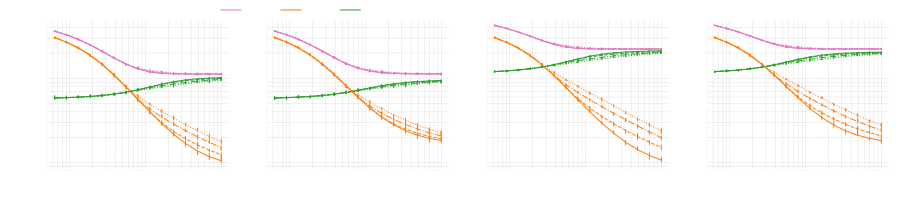
\includegraphics[width=0.6\textwidth]{Assets/feature_combinations_alpha_sweep.pdf}

}


% Title, author and affiliations section
\titlebox{
    \title{A High Dimensional Statistical Model for Adversarial Training: Geometry and Trade-Offs}  
    }
% End of title stuff
    
%% Central box with traditional content
\centerbox{
\begin{multicols}{3}

\section{Problem Setup}

\textbf{Binary Classification Setting}:
\begin{itemize}
    \item Training data \(\mathcal{D} = \qty{(\x_\datidx, y_\datidx)}_{\datidx=1}^{n}\in\mathbb{R}^{d}\times\{-1,+1\}\)
    \item Probit model with noise parameter $\tau > 0$
    \item High-dimensional limit: $d,n \to \infty$ with fixed $\alpha = n/d$
    \item Structured data with block features: covariance matrices $\Sigmax, \Sigmadelta, \Sigmaupsilon, \Sigmatheta$ are block diagonal with $k$ blocks of sizes $d_1, \dots, d_k$
\end{itemize}

\textbf{Metrics of Interest}:
\begin{itemize}
    \item Generalisation Error:
    \begin{equation}
        \generr = \EEb{y,\x}{ \mathbb{1}(y \neq \hat{y} (\what, \x)) }
    \end{equation}
    
    \item Adversarial Generalisation Error:
    \begin{equation}
        \advgenerr = \EEb{y,\x}{
            \max_{\norm{\vecdelta}_{\Sigmaupsilon^{-1}} \leq \advgencost} \mathbb{1}(y \neq \hat{y} (\what, \x + \vecdelta))
        }
    \end{equation}
    
    \item Boundary Error:
    \begin{equation}
        \advgenerr = \generr + \bounderr
    \end{equation}
    where $\bounderr$ are the attackable samples.
    
    \item Usefulness and Robustness:
    \begin{align}
        \usefulmetric_{\wstar}
        &= \frac{1}{\sqrt{d}} \mathbb{E}_{\x, y}[y \wstar^\top \x ] \label{eq:mt-usefulness-def} \\
        \robustmetric_{\wstar} &= \frac{1}{\sqrt{d}} \EEb{\x, y}{
            \inf_{\norm{\vecdelta}_{\Sigmaupsilon^{-1}}  \leq \advgencost} y \wstar^\top ( \x + \vecdelta)
        } \label{eq:mt-robustness-def}
    \end{align}
\end{itemize}

\textbf{Adversarial ERM}:
\begin{equation}
    \sum_{\datidx = 1}^{n} 
    g \qty(
        y_\datidx \frac{\w^\top \x_\datidx}{\sqrt{d}} 
        - \advtrainingcost \frac{\sqrt{\w^\top \Sigmadelta \w}}{\sqrt{d}} 
    ) 
    + r(\w)
\end{equation}

\section{Main Result}

\textbf{Theorem:} Adversarial generalization errors are \textit{provably} characterized by a system of 8 order parameters $(m, q, V, P, \hat{m}, \hat{q}, \hat{V}, \hat{P})$ and an additional parameter \(A\) through:

\begin{align}
    \generr &= \frac{1}{\pi} \arccos \qty( 
    {
        m / \sqrt{ (\rho + \tau^2) q}
    } 
    ) \\
    \bounderr &= \!
    \int_{0}^{\advgencost \frac{\sqrt{A}}{\sqrt{q}}} \!\!\!\!
    {\textstyle
        \erfc\left( \frac{ -\frac{m}{\sqrt{q}} \nu}{\sqrt{2 \qty(\rho + \tau^2 - m^2 / q)}} \right) 
        \!\! \frac{e^{-\frac{\nu^2}{2}}}{\sqrt{2\pi}} \dd{\nu}
    }
    \label{eq:adv-error-theorem-overlap}
\end{align}

\section{Implications}

\subsection{Trade-off between Usefulness and Robustness}:

\begin{itemize}
    \item Usefulness relates to generalisation error
    \item Robustness relates to boundary error
    \item Trade-off emerges when protecting useful but non-robust features
\end{itemize}

\textbf{Key Bounds}:

\begin{equation}
    \generr
    \geq
    \frac{1}{\pi} \arccos( \sqrt{\frac{\pi}{2 \rho}} \usefulmetric_{\wstar} )
    \label{eq:bound-gen-error}
\end{equation}

\begin{equation}
    \bounderr \leq 2 \mathrm{T}\qty( \advgencost \mathcal{A} \, \mathcal{B}, \mathcal{A}^{-1} ) - \frac{1}{\pi} \arctan( \mathcal{A}^{-1} ) - \frac{1}{\pi} \erf\qty( \frac{\advgencost \mathcal{B}}{\sqrt{2}} ) \erfc\qty( \frac{\advgencost \mathcal{A} \, \mathcal{B}}{\sqrt{2}} )
    \label{eq:bound-boundary-error}
\end{equation}

\subsection{Directional Defences and structured data}

\textbf{Key Finding:} The choice of defense strategy significantly impacts adversarial performance:

\begin{center}
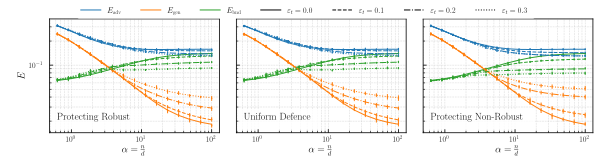
\includegraphics[width=0.3\textwidth]{Assets/defence_sweep.pdf}
\postercaption{Impact of different defense strategies on generalization ($\generr$) and boundary ($\bounderr$) errors}
\end{center}

\begin{itemize}
    \item \textbf{Defending robust features}: Low $\generr$ but high $\bounderr$
    \item \textbf{Uniform defense}: Better balance, improves overall $\advgenerr$
    \item \textbf{Defending non-robust features}: Increases $\generr$ while decreasing $\bounderr$
\end{itemize}

\textbf{Analytical Result:} For structured data with two feature blocks, we prove that protecting non-robust features:
\begin{itemize}
    \item Always increases $\generr$ and decreases $\bounderr$
    \item Can improve $\advgenerr$ when attack size is small enough
\end{itemize}

\subsection{Tradeoff directions and innocuous directions}

\textbf{Key Insight:} The geometry of features determines whether adversarial training leads to a trade-off:

\begin{center}
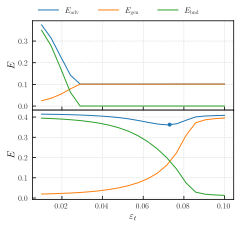
\includegraphics[width=0.3\textwidth]{Assets/optimal_defense.pdf}
\postercaption{Impact of adversarial training on features with different geometries}
\end{center}

\textbf{Two Distinct Cases:}

\begin{itemize}
    \item \textbf{Innocuous Features} (orthogonal to teacher):
    \begin{itemize}
        \item Attack can be completely neutralized
        \item $\advgenerr \to \generr$ as $\advtrainingcost$ increases
        \item $\bounderr \to 0$ with sufficient training
    \end{itemize}
    
    \item \textbf{Trade-off Features} (aligned with teacher):
    \begin{itemize}
        \item Fundamental trade-off between $\generr$ and $\bounderr$
        \item Optimal performance at specific $\advtrainingcost$
        \item Requires careful hyperparameter tuning
    \end{itemize}
\end{itemize}

\subsection{Data Dependent Regularisation}

\textbf{Key Finding:} Adversarial training can be approximated as a data-dependent regularisation:

\begin{center}
    \includegraphics[width=0.3\textwidth]{Assets/gen_lambda_optimal_sweep_alpha.pdf}
    \postercaption{Adversarial training is not just an $\ell_2$ regularisation}
\end{center}

\begin{center}
\includegraphics[width=0.3\textwidth]{Assets/effective_regularisation.pdf}
\postercaption{Learning curves for adversarial training (top) and its regularisation approximation (bottom)}
\end{center}

\textbf{Approximate Loss:}
\begin{equation}
    \sum_{\datidx = 1}^{n} 
    g \Big( y_\datidx \frac{\w^\top \x_\datidx}{\sqrt{d}} \Big) 
    + \tilde{\lambda}_1 \sqrt{\w^\top \Sigmadelta \w} + \tilde{\lambda}_2 \w^\top \Sigmadelta \w
\end{equation}

\textbf{Key Properties:}
\begin{itemize}
    \item \textbf{Not just $\ell_2$}: Performance depends on $\advtrainingcost$ even with optimal $\lambda$
    \item \textbf{Effective Regularisation}: is a directional \(\sqrt{\ell_2} + \ell_2\) regularisation
    \item \textbf{Non-sparse}: $\sqrt{\ell_2}$ term provides linear scaling in the norm of the student vector without sparsity
\end{itemize}

\section{Acknowledgements}

Bruno Loureiro acknowledges support from the \textit{Choose France - CNRS AI Rising Talents} program, and Florent Krzakala from the Swiss National Science Foundation grant SNFS OperaGOST  (grant number $200390$).

\end{multicols}
}




% End of central box

% Bottom box with QR code
\bottombox{
    %% QR code
    \qrcodecommand{https://arxiv.org/abs/2402.05674}{

    Kasimir Tanner
    \newline
    Matteo Vilucchio
    \newline
    Bruno Loureiro
    \newline
    Florent Krzakala
    \newline

}
}{
    % Comment out the line below out to hide logo
    \hfill\bottomboxlogo{Assets/EPFL_Logo_Digital_RGB_PROD.png} % \hfill shifts the logo across so it meets the right hand side margin
    % Note that \bottomboxlogo takes an optional width argument. It defaults to the following: 
    % \hfill\bottomboxlogo[width=\textwidth]{<path_to_image_file>} 
    % where \textwidth is actually the width of a minipage which is defined in the \bottombox command of
    % betterportaitposter.cls It's a standard \includegraphics command in there, so easy to change if 
    % you need to add a border etc.
}
% End of bottom box



\end{document}